\section{Arquitectura física del sistema}
\paragraph\indent
\textbf{Arquitectura del sistema:} Es la tecnología que proporciona al usuario final el acceso transparente a las aplicaciones, datos, servicios de cómputo o cualquier otro recurso a través de la organización en múltiples plataformas. El modelo soporta un medio ambiente distribuido en el cual los requerimientos de servicio hechos por estaciones de trabajo inteligentes o clientes resultan en un trabajo realizado por otros computadores llamados servidores.

\textbf{Cliente:} Es el que inicia un requerimiento de servicio. El requerimiento inicial puede convertirse en múltiples requerimientos de trabajo. La ubicación de los datos o de las aplicaciones es totalmente transparente para el cliente.

\textbf{Servidor:} Es cualquier recurso de cómputo dedicado a responder a los requerimientos del cliente. Los servidores pueden estar conectados a los clientes a través de redes LAN o WAN para proveer de múltiples servicios a los clientes tales como impresión, acceso a bases de datos, fax, procesamiento de imágenes, etc.
\paragraph\indent
La arquitectura cliente-servidor es un modelo de aplicación distribuida en el que las tareas se reparten entre los servidores, que proveen de recursos o servicios, y los clientes, que demandan por estos recursos y servicios. Si un cliente realiza peticiones a otro programa es el servidor quien le da una respuesta.

\subsection{Ventajas}
\begin{itemize}
	\item Centralización del control: los accesos, recursos y la integridad de los datos son controlados por el servidor de forma que un programa cliente defectuoso o no autorizado no pueda dañar el sistema. Esta centralización también facilita la tarea de poner al día datos u otros recursos.
	\item Escalabilidad: se puede aumentar la capacidad de clientes y servidores por separado. Cualquier elemento puede ser mejorado en cualquier momento, o se pueden añadir nuevos nodos a la red (clientes y/o servidores).
	\item Fácil mantenimiento: al estar distribuidas las funciones y responsabilidades entre varios ordenadores independientes, es posible reemplazar, reparar, actualizar, o incluso trasladar un servidor, mientras que sus clientes no se verán afectados por ese cambio. Esta independencia de los cambios también se conoce como encapsulación.
	\item Tecnologías: Existen tecnologías, suficientemente desarrolladas, diseñadas para el paradigma de C/S que aseguran la seguridad en las transacciones, la amigabilidad de la interfaz, y la facilidad de empleo.
\end{itemize}

\subsection{Desventajas}
\begin{itemize}
	\item Tráfico: La congestión del tráfico ha sido siempre un problema en el paradigma de C/S. Cuando una gran cantidad de clientes envían peticiones simultáneas al mismo servidor, puede ser que cause muchos problemas para éste.
	\item Robustez: El paradigma de C/S clásico no tiene la robustez de una red P2P. Cuando un servidor está caído, las peticiones de los clientes no pueden ser satisfechas.
	\item El software y el hardware de un servidor son generalmente muy determinantes. Un hardware regular de un ordenador personal puede no poder servir a cierta cantidad de clientes. Normalmente se necesita software y hardware específico, sobre todo en el lado del servidor, para satisfacer el trabajo.
	\item El cliente no dispone de los recursos que puedan existir en el servidor. Por ejemplo, si la aplicación es una Web, no podemos escribir en el disco duro del cliente o imprimir directamente sobre las impresoras sin sacar antes la ventana previa de impresión de los navegadores.
\end{itemize}

\section{Diagrama de despliegue}
Un diagrama de despliegue modela la arquitectura en tiempo de ejecución de un sistema. Esto muestra la configuración de los elementos de hardware y muestra cómo los elementos y artefactos del software se trazan en esos nodos.
\begin{figure}[H]
		\centering
		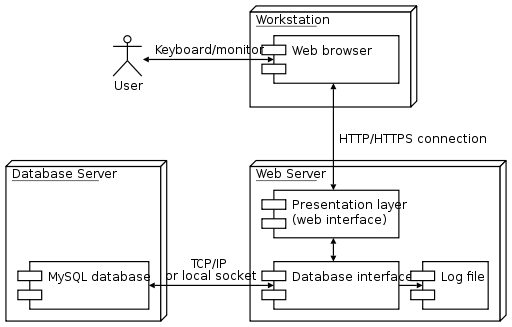
\includegraphics[width=\textwidth,height=0.95\textheight,keepaspectratio]{Extras/diagramaDespliegue}
		\caption{Diagrama de despliegue}
	\label{fig:diagramaDespliegue}
	\end{figure}